%%%%%%%%%%%%%%%%%%%%%%%%%%%%%%%%%%%%%%%%%%%%%%%%%%%%%%%%%%%%%%%%%%%%%%%%%%%%%%%%
% simulation.tex: Chapter on MC production:
%%%%%%%%%%%%%%%%%%%%%%%%%%%%%%%%%%%%%%%%%%%%%%%%%%%%%%%%%%%%%%%%%%%%%%%%%%%%%%%%
\chapter{Simulation}
\label{simulation_chapter}
%%%%%%%%%%%%%%%%%%%%%%%%%%%%%%%%%%%%%%%%%%%%%%%%%%%%%%%%%%%%%%%%%%%%%%%%%%%%%%%%

%%%%%%%%%%%%%%%%%%%%%%%%%%%%%%%%%%%%%%%%%%%%%%%%%%%%%%%%%%%%%%%%%%%%%%%%%%%%%%%%
In order to predict spectra at the near and the far detectors to compare predictions with
actual data one needs to simulate neutrino interactions in the detectors relying on
known physics models and theories of how particles are produced, how they travel and interact
with detector material. The simulation process in NOvA starts with protons hitting
the NuMI target and finishes with APD readouts and analog to digital converters. Side simulation
packages or custom NOvA software are used in every step, output information on every step is
used as input data for the following step
\begin{itemize}
\item Beam simulations: The FLUGG simulation package combines FLUKA \cite{FLUKA} with GEANT4 \cite{GEANT4}.
Geometries of the target hall and detectors are encoded in GEANT4, and the proton interactions
and downstream particle decays are simulated with FLUKA.
\item Neutrino interactions: The neutrino flux generated in the previous step is input into
the GENIE \cite{GENIE} package, which simulates neutrino-nucleus interactions inside the
detectors. In each event GENIE produces a list of particles leaving the nucleus.
\item Particle propagation: Particles produced by GENIE are propagated through the detector,
and their interactions with the detector materials and decays are simulated by GEANT4. Amount of
energy deposited in every cell is passed to the last step.
\item Electronic signal: Deposited energy in the cell is converted to a light by the scintillator;
then light travels through the fiber to an APD and analog to digital converter. This step is
simulated by NOvA custom software \cite{NovaSim}.
\end{itemize}
All of these parts are briefly discussed here.

\section{Beam Simulation}
The beam simulation estimates the neutrino flux into both detectors, and is accomplished using FLUKA and
GEANT4 via the FLUGG interface. A detailed geometry of the target hall and target, the collimator, two
focusing horns and the decay pipe is implemented in GEANT4, and the particle simulation is handled by
FLUKA. The FLUKA package simulates 120 GeV protons which hit the graphite target, which yield hadronic 
showers of secondary particles that are directed by the horns into the decay pipe where they decay to 
neutrinos. All the proton interaction information whose daughter particles produce a
neutrino is saved providing a way to study beam uncertainties related to particle production models. 

The simulation outputs files which describe neutrino flux in terms of neutrino parent particles, 
flavour, energy and direction of motion.

\section{Simulation of Neutrino Interactions}
The neutrino interactions between ND and FD materials is simulated using GENIE. GENIE is developed
by the experimental physics community, and is widely used as a neutrino Monte Carlo simulator for experiments due
to its flexibility to simulate different target materials, and the accuracy of its results over a large
range of neutrino energies which spans from MeV to PeV. As mentioned above GENIE gets a result of neutrino 
flux simulation from a previous step and convolutes it with neutrino interaction cross sections.

The neutrino energy spectrum expected in NOvA measurements overlaps
with the energy regions of several neutrino interaction models, all of which are implemented in GENIE.
These models include Quasi-Elastic scattering (QE), deep-inelastic scattering (DIS), baryon resonance
production (RES) as well as meson exchange current (MEC) which dominates in 2 particle - 2 hole (2p-2h) 
effect. The physics behind the models is complicated, however on the qualitative level the QE interaction 
represents scattering off a single nucleon, the MEC interaction means scattering off a pair of nucleons, 
the RES process produces an excited nucleus, and the DIS interaction between a neutrino and a nucleus can 
disintegrate the nucleus\footnote{This happens only when the energy transferred to a nucleus is 
sufficiently large}.

\begin{figure}[t!]
\begin{subfigure}[t]{.5\textwidth}
  \centering
  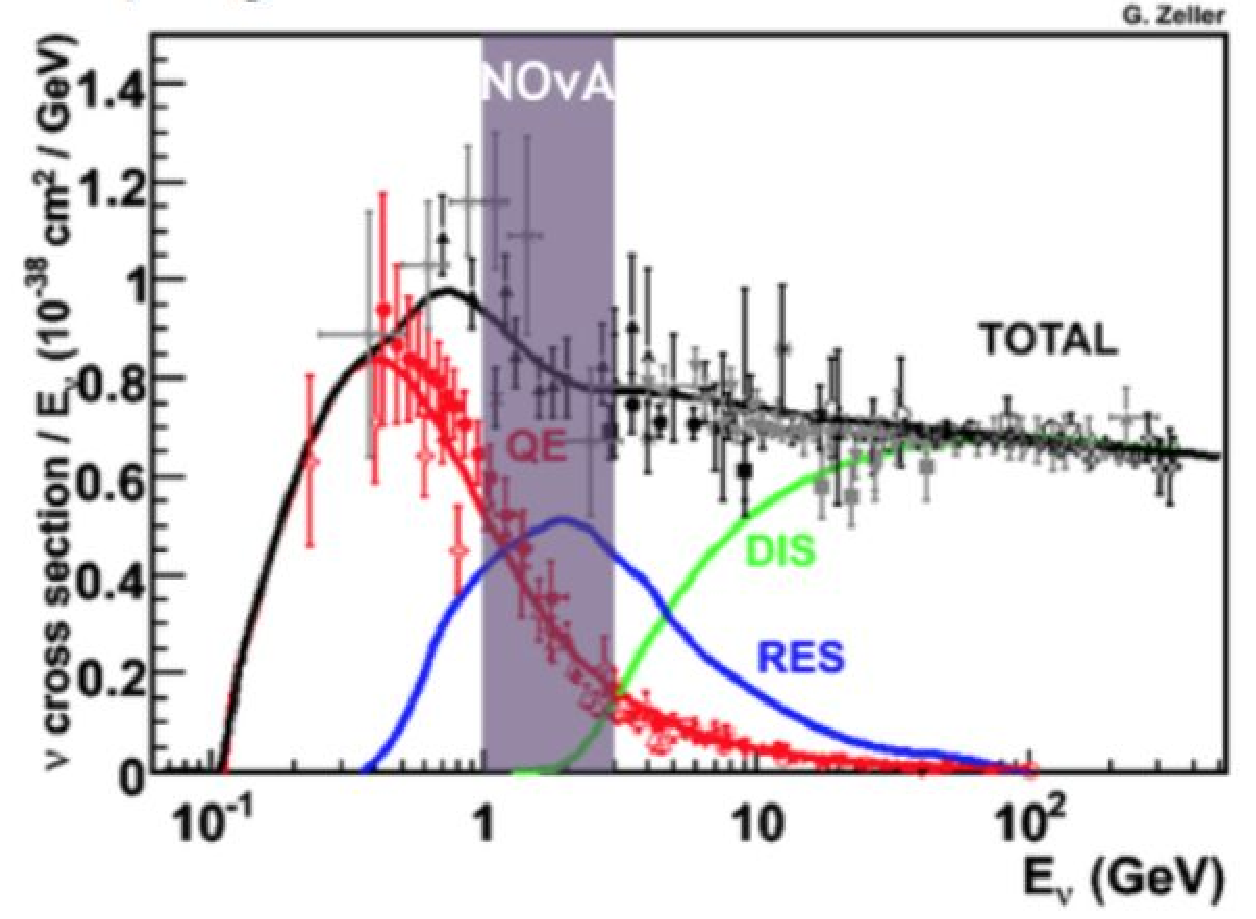
\includegraphics[width=0.85\linewidth]{figures/nu_channels.pdf}
  \caption{Neutrino cross section energy dependence for QE, RES and DIS interactions overlapped with 
	NOvA energy region used for the oscillation analysis.}
  \label{fig:NovaEReg}
\end{subfigure}%
~
\begin{subfigure}[t]{.5\textwidth}
  \centering
  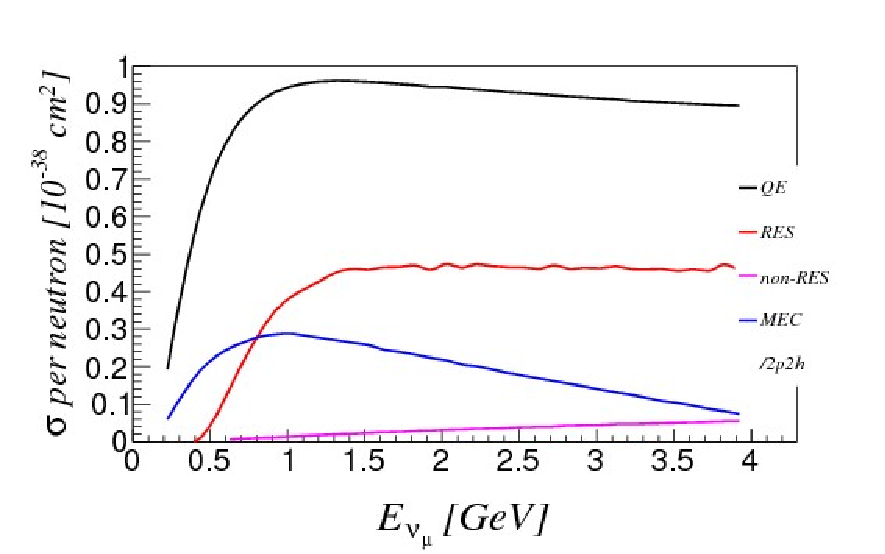
\includegraphics[width=1.1\linewidth]{figures/mec_xsec.pdf}
  \caption{Neutrino cross section energy dependence used in GENIE neutrino generator.}
  \label{fig:mecXsec}
\end{subfigure}
\caption{Neutrino cross sections.}
\label{fig:simPlots}
\end{figure}

Based on the left hand side of \ref{fig:NovaEReg}, the typical energy regions of QE, RES and DIS neutrino 
interactions overlap with the NOvA energy domain. These three types of neutrino scattering are implemented 
in GENIE based on the Llewellyn-Smith model \cite{QE}, Rein-Sehgal model \cite{RES} and effective leading 
order model with Bodek and Yang modifications \cite{DIS} for QE, RES and DIS respectively. MEC process, 
which is included in GENIE as semi-empirical model, is described in \cite{MEC}.

\section{Particles Propagation and Cerenkov Light}
After GENIE is done with its part of simulation, or in other words, the list of particles which leave 
the nucleus with their energies, momenta and initial positions is ready, now one needs to propagate them
through the detector material and simulate the energy deposition, interaction and decay. NOvA experiment
uses GEANT4 \cite{GEANT4} simulation package for this step. Besides the list of particles, GEANT4 takes
another input, namely geometry of the detector and its surrounding. Detailed information about blocks 
positions, cell structure and materials they made of, scintillator composition, concrete and steel support
structure around the detectors is encoded in special geometry files.

The way GEANT4 propagates particles is done in the following manner. For each particle at each step of the 
trajectory it is decided with appropriate probability what particle should do next - move forward and deposit 
some energy, interact and scatter of particles that represent detector components, or decay. As a particle
propagates further it loses its kinetic energy and as soon as particle's kinetic energy is less than 100 eV
propagation stops. GEANT4 saves these trajectory steps as a list of particle positions, energy and momenta 
for the next step of simulation chain. 

Before the final detector response could be simulated it is necessary to determine how much light was produced
in the scintillator and what fraction of it was collected by the wave-shifting fiber and transported to the 
readout electronics. As a matter of fact, amount of light produced by the scintillator is not linearly 
proportional to amount of deposited energy due to a finite number of scintillator centres along the particle
trajectory in the cell. The effect is know as Birks suppression \cite{birks}. If $\frac{dL}{dx}$ is light 
output per unit length and $\frac{dE}{dx}$ is amount of deposited energy then Birks law reads
\be
\frac{dL}{dx} = L_0 \frac{\frac{dE}{dx}}{1 + k_B\frac{dE}{dx}}, 
\ee
where $L_0$ and $k_B$ are constants which depend on scintillator. Parameter $k_B$ is tuned using muon and 
protons tracks in the Near Detector.

Another phenomena which plays a significant role in light production is Cerenkov effect \cite{cerenkov}. 
This effect was observed in a bottle of water subjected to radioactive bombardment. Charged particle while
moving through the liquid with velocity greater than the phase velocity of light emits light and this emission 
is simulated in NOvA experiment. The following formula is used to predict the number of Cerenkov photons produced
per distance traveled at a given wavelength 
\be
\frac{dN_\gamma}{dxd\lambda} = \frac{2\pi\alpha z^2}{\lambda^2}\Big(1 - \frac{1}{\beta^2n^2(\lambda)}\Big),
\ee
where $\alpha$ is fine-structure constant, $z$ is charge of moving particle in units of $e$, $n(\lambda)$ is 
refraction index and $\beta$ is particle's velocity in units of $c$.

%However, more careful approach to the problem
%of particle propagation through scintillator was carried out by Chou \cite{chou} and additional correction was
%introduced to the Birks law. NOvA experiment utilizes this correction - 
%\be
%\frac{dL}{dx} = L_0 \frac{\frac{dE}{dx}}{1 + k_B\frac{dE}{dx} + k_C\Big(\frac{dE}{dx}\Big)^2}.
%\ee
%Parameters $k_B$ and $k_C$ are tuned using muon and protons tracks in the Near Detector.

\section{Light propagation and signal to store}
The last simulation step is done using custom NOvA software that is split into two parts - light
propagation to the readout electronics, and the signal measurement made by the electronics. Although in practice cells could 
be different from each other (horizontal cells are not exactly horizontal because of their length - cells could be
slightly bent, especially in the far detector. Not exact horizontality also leads to small bubbles of air are
being trapped inside the cells) in simulations it is assumed that all cells are identical.

\subsection{Light propagation}
Assuming all cells are equivalent, a ray-tracing model is used to estimate how many photons were trapped by
each WLS fiber. The following characteristics of detector components were measured in bench experiments, and
used in light propagation simulations:
\begin{itemize}
\item characteristic scintillator emission time - 9 ns
\item scintillator index of refraction - 1.46
\item reflectivity of the cell walls - 87.7\%
\item photon capture length\footnote{Probability to capture a photon $P \sim e^{x/L}$, where
$x$ is distance between the point where the photon was produced and the fiber, $L$ is capture length.} - 30.66 cm
\end{itemize}
The resulting template is shown on \ref{fig:Coll_rate}. This template is used to determine the number of photons 
trapped in WLS fiber. To simulate what fraction of photons reaches the APD
half of photons are sent in opposite directions around the fiber. There are some fraction on photons which is 
absorbed or get out of fiber, and the effect is accounted for in simulation by using attenuation curve which was 
measured in bench tests. Before the last simulation step starts, the number of photoelectrons created in each APD
is determined by taking into account APD's quantum efficiency and additional Poisson smearing.
\begin{figure}
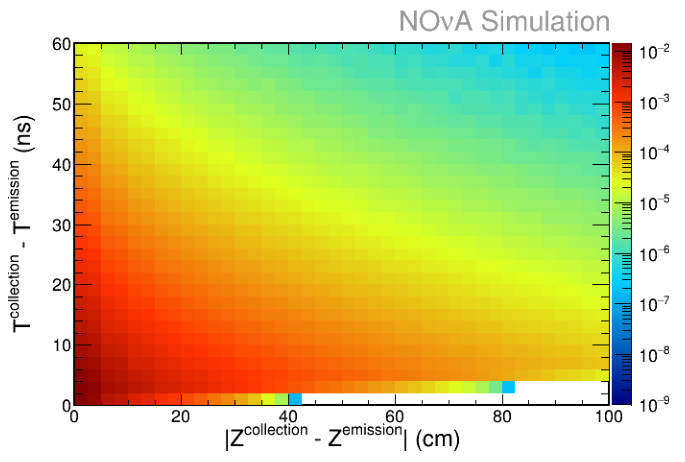
\includegraphics[width=1.0\textwidth]{figures/Coll_rate.png}
\centering
\caption{The collection rate of scintillator photons by a wavelength shifting fiber loop relative to the position 
	and time where and when the energy was deposited.} \label{fig:Coll_rate}
\end{figure}
\begin{figure}[t!]
\begin{subfigure}[t]{0.9\textwidth}
  \centering
  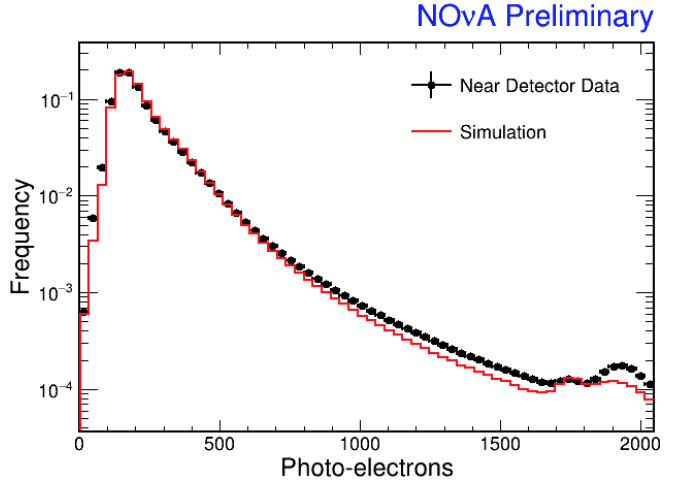
\includegraphics[width=0.9\linewidth]{figures/AttenuationND.png}
  \caption{Near Detector}
  \label{fig:attND}
\end{subfigure}
\vspace{0.5cm}
\newline
\begin{subfigure}[t]{0.9\textwidth}
  \centering
  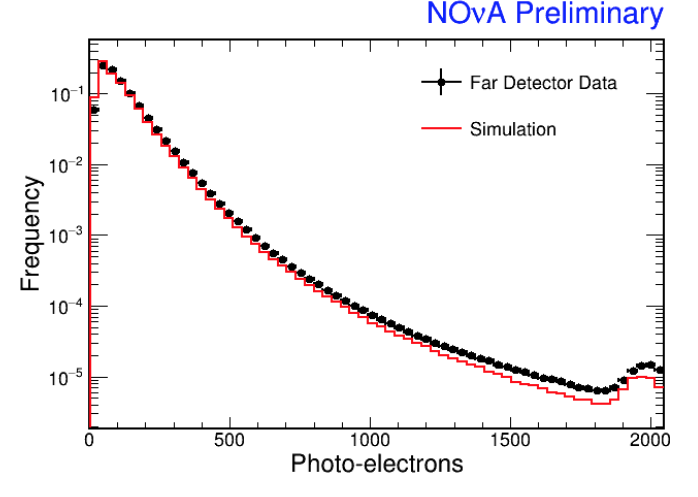
\includegraphics[width=0.9\linewidth]{figures/AttenuationFD.png}
  \caption{Far Detector}
  \label{fig:attFD}
\end{subfigure}
\caption{Attenuation curves for the near and the far detectors. Data points are detectors response to cosmic ray
	muons while simulation curves are results of bench experiments.}
\label{fig:att}
\end{figure}

\subsection{Electronics}
\begin{wrapfigure}{r}{0.5\textwidth}
\vspace{-20pt}
  \begin{center}
    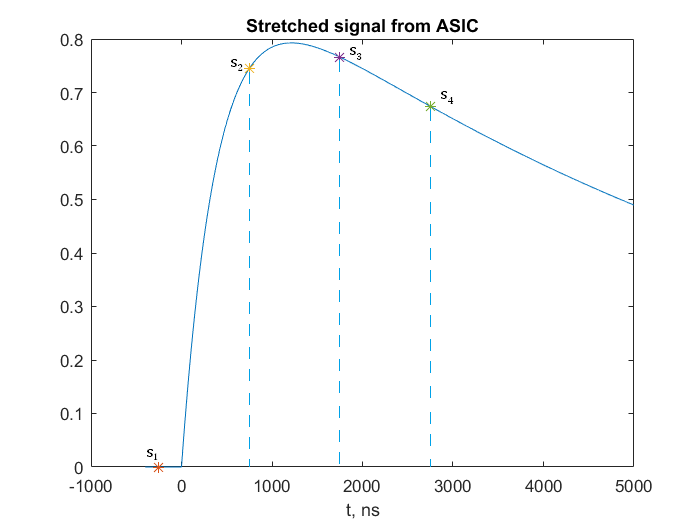
\includegraphics[width=0.48\textwidth]{figures/digit_scheme.png}
  \end{center}
\vspace{1mm}
\caption{Schematics of digitization}
\end{wrapfigure}
Photo-electron signal in the APD created in the previous step have to be digitized to finalize the simulation
of the cell hit. As an APD impulse is too short, first it is stretched in the Application Specific Integrated 
Circuit (ASIC) by the CR-RC circuit. The response of the ASIC to a charged impulse has the following form
\be
f(t) \sim e^{-\frac{t-t_0}{F}} - e^{-\frac{t-t_0}{R}},
\ee
where $t_0$ is the time when pulse was created by APD, F and R are the fall time and rise time of the CR-RC 
circuit. And as was mention in chapter \ref{experiment_chapter} the signal value is split into 4096 possible
values and only 4 last ADCs - value of the digitization sample - is stored when the difference $ADC_i - ADC_{i-3}$
is greater then a threshold. 
At this point the simulation files have the same structure\footnote{Of course plus additional information about type 
of neutrino information, resulting particles' momenta and energies etc.} as the data files.
The next step in NOvA analysis is to reconstruct high level information about recorded or simulated events
with the help of reconstruction algorithms which are the same for the real data and simulation.
